%!TeX root=../main.tex
\فصل{آشنایی با \متن‌لاتین{LoRa}}
\قسمت{مقدمه}
اینترنت اشیاء\پانویس{IOT: Internet of things} واژه‌ای که این روزها برسر زبان بسیاری از افراد است. بدون شک این تکنولوژی آینده فناوری اطلاعات را در دست خواهد گرفت. جهت پیاده سازی این تکنولوژی زیرساخت‌های خوبی لازم است چرا که داده ها در این تکنولوژی بسیار زیاد است و همچنین دیگر تکنولوژی هایی چون \متن‌لاتین{Wi-Fi} و \متن‌لاتین{Li-Fi} جهت ارتباطات جواب گوی این حجم انتقالات نیست و باید به فکر تکنولوژی های جایگزین بود.

در حوزه اینترنت اشیاء، فاکتورهای بسیاری از جمله هزینه \متن‌لاتین{Node}ها، هزینه شبکه، طول عمر باتری، نرخ اطلاعات، تاخیر، مسافت پوشش‌دهی و محل استقرار اهمیت پیدا می‌کند. هیچ فناو
ری‌ به‌تنهایی قادر نیست به‌طور همزمان نسبت به تمامی بخش‌ها پاسخ‌گو باشد اما در این میان، از فناوری \متن‌لاتین{LoRa} به‌دلیل داشتن بیشترین ویژگی مثبت، می‌توان استفاده کرد.

شبکه \متن‌لاتین{LoRaWAN} یک پروتکل توان پایین با برد وسیع\پانویس{LPWA} است که به‌خصوص برای دستگاه های بیسیم در اینترنت اشیا طراحی شده است و در سطح شبکه های منطقه ای، ملی یا جهانی میتواند عمل کند. معماری شبکه \متن‌لاتین{LoRaWAN} به صورت توپولوژی ستاره یا استار میباشد که در آن گیتوی‌ها پیام ها را بین دستگاه های پایانی و سرور مرکزی شبکه انتقال می دهند. گیتوی‌ها مانند یک پل نامرئی عمل می کنند و از طریق اتصالات استاندارد آی پی به سرور در شبکه متصل می شوند، به سادگی بسته‌های RF را به بسته‌های IP تبدیل می کنند و بلعکس. همان‌طور که در شکل 1 مشاهده می‌کنید، تعداد زیادی \متن‌لاتین{Node} می‌توانند به گیتوی متصل شوند که معمولا این \متن‌لاتین{Node}ها به سنسورهایی مثل سنسور دود، رطوبت، دما و ... متصل هستند و اطلاعات این سنسورها را به گیتوی مخابره می‌کنند.

به‌طورکلی در این پروژه مصرف پایین انرژی به دلیل استفاده از سیستم باطری و پنل خورشیدی بسیار اهمیت دارد. استفاده از شبکه تلفن همراه\پانویس{The Global System for Mobile Communications (GSM)} به‌عنوان راه‌حلی ابتدایی برای ارتباط بی‌سیم، علاوه بر نداشتن صرفه اقتصادی مصرف انرژی زیادی را به سیستم تحمیل می‌کند. همچنین تضمینی برای وجود پوشش شبکه تلفن همراه در مناطقی که قرار است داده‌های جوی از آن جمع‌آوری شود وجود ندارد. ازاین‌رو بهترین رویکرد استفاده از گیرنده و فرستنده‌های رادیویی در باندهای فرکانسی بدون نیاز به مجوز (\متن‌لاتین{ISM}) است. از میان گزینه‌های موجود ماژول‌های لورا\پانویس{\متن‌لاتین{LoRa} (Long Range)} به لطف مدولاسیون \متن‌لاتین{\متن‌لاتین{CSS}\پانویس{Chirp Spread Spectrum}} که از آن بهره می‌برند دارای مصرف توان پایین، ناحیه پوشش وصیع و نفوذپذیری مناسبی هستند که کاملاً با نیازهای ما سازگار است. در ادامه به بررسی و مقایسه این تکنولوژی با سایر گزینه‌های موجود پرداخته می‌شود.

\قسمت{جنبش جهانی شبکه اشیاء (\متن‌لاتین{TTN:The Things Network})}
 با هدف ایجاد یک شبکه جهانی باز و عمومی (شهر هوشمند) ، غیر متمرکز و مبتنی بر همکاری جمعی، مدتی است که با سرعت بالا در سراسر جهان در حال فراگیر شدن است. به این صورت که تعدادی دروازه در نقاط مختلف کشور نصب می‌شود و به توسعه‌دهندگان صنعت اینترنت اشیا اجازه داده می‌شود که محصولات خود را بطور رایگان به این درگاه ها متصل کنند و پس از ایجاد حساب در سایت \متن‌لاتین{The Things Network}\پانویس{www.thethingsnetwork.org} می‌توانند از هر نقطه‌ای محصولات خود را کنترل کنند. هر دروازه \متن‌لاتین{LoRa}، توانایی پشتیبانی هزاران \متن‌لاتین{Node} را دارد. این درگاه‌ها می‌توانند تا شعاع 15 کیلومتری را پوشش دهند. در شکل \رجوع{fig:loraGlobal}، نقاط پوشش‌دهی \متن‌لاتین{LoRaWAN} را در سطح جهانی مشاهده می‌کنید.
 
\begin{figure}[!h]
	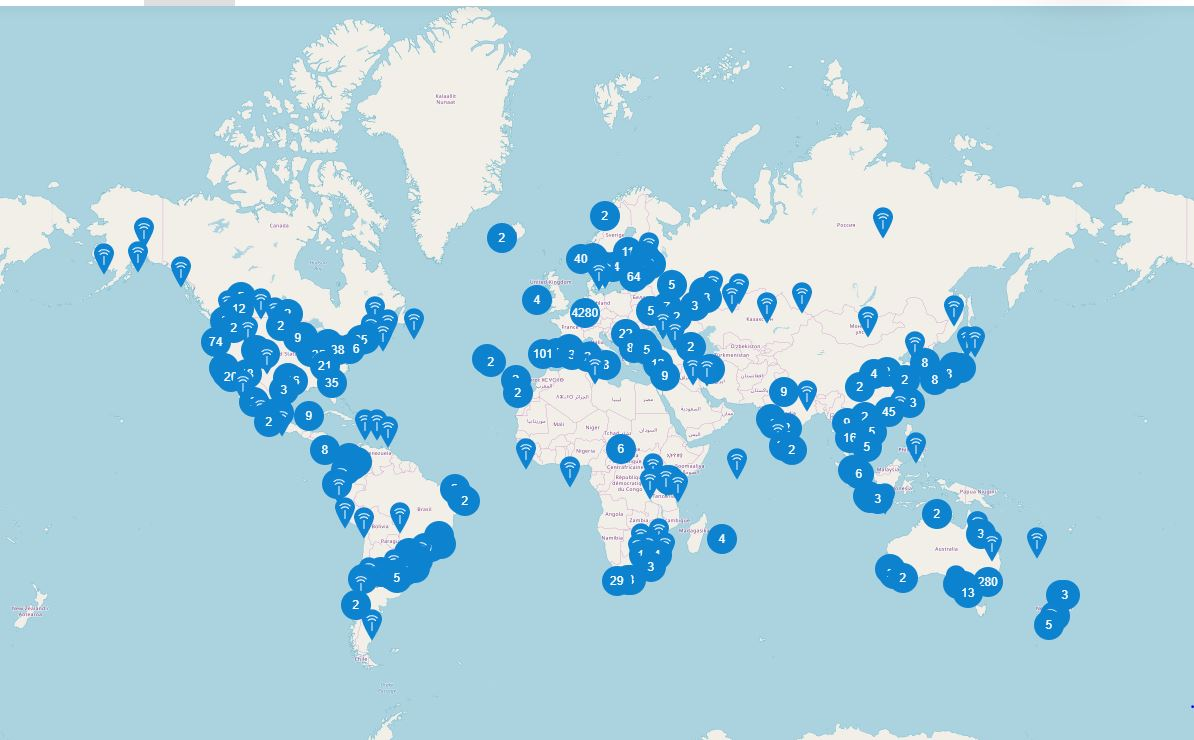
\includegraphics[width=\linewidth]{Assets/loraGlobal.png}
	\caption{نقاط پوشش‌دهی \متن‌لاتین{LoRaWAN} در سطح جهانی.}
	\label{fig:loraGlobal}
\end{figure}

شبکه اشیا ابتدا در شهر آمستردام هلند آغاز به کار کرد و در مدت چهار هفته، کل این شهر تحت پوشش شبکه اینترنت اشیا قرار گرفت. کشور ایران نیز پیش‌تر درخواست خود را برای پیوستن به این شبکه اعلام کرده و در سال 1395 موفق به کسب موافقت برای راه‌اندازی شبکه اشیا در تهران شد. اولین درگاه، در همان سال در منطقه نارمک تهران نصب شد. این نخستین درگاه شبکه اشیاء در خاورمیانه است و ایران را در کنار کشورهای دارای این فناوری قرار می‌دهد\مرجع{mehrnews:lora}.

مخاطب اصلی این شبکه را اپراتورهای ارتباطی، استارتاپ‌ها و کسب و کارهای مرتبط با فناوری اطلاعات است. این شبکه در واقع شبکه‌ای غیرانتفاعی است که به‌جز هزینه‌های پایین سرمایه‌گذاری اولیه، اجرایی و نگهداری، هزینه دیگری در بر ندارد و هدف از توسعه آن درآمدزایی مستقیم نیست. چنین شبکه‌ای می‌تواند بستری شود تا شرکت‌ها و افراد خلاق با ارائه خدمات نوآورانه خود، از آن‌ها کسب ارزش کنند. 

تفاوت ارائه خدمات ارائه خدمات بر روی این شبکه با سرویس‌هایی که از طریق شبکه‌های ارتباطی موبایل ارائه می‌شود، توان مصرفی بسیار پایین و در مقابل پوشش گسترده آن است. از سوی دیگر، به هیچ عنوان هزینه این اتصال قابل قیاس با اتصال اشیاء از طریف سیم‌کارت موبایل نیست. برای مثال این شبکه می‌تواند در حوزه خدمات شهری برای هوشمندسازی پارکینگ‌ها، کنتورهای هوشمند، اتصال حسگرهای انبوه برای اندازه‌گیری آلودگی، رطوبت و... و نهایتا کاهش ترافیک و میزان آلودگی کاربرد داشته باشد. به عبارتی کاربرد اصلی این شبکه را توسعه دهندگان تعریف می‌کنند و بسته به نیاز و خلاقیت خود می‌توانند به کاربردهایی بیندیشند که تا کنون ارائه آن‌ها ممکن نبوده و یا هزینه زیادی در پی داشته است. با راه‌اندازی این زیرساخت، شرکت‌ها دیگر مجبور نیستند که به صورت جزیره‌ای شبکه ایجاد کنند و به جای آن می‌توانند بر روی خدمات مناسب تمرکز کرده و از آن‌ها ارزش‌آفرینی کنند.

این شبکه قرار نیست رقیب شبکه‌های کنونی ثابت و سیار باشد، در حقیقت شبکه اشیاء آمده است تا جای خالی خود را پر کند و به عنوان شبکه‌ای مکمل این دو عمل کند. این امکان را فراهم می‌کند تا کاربردهایی که پیش‌تر به دلیل هزینه‌های بالای اتصال، امکان بروز و ظهور نمی‌یافتند، اکنون عملیاتی شوند.  ایجاد چنین شبکه‌ای می‌تواند بستری شود تا شرکت‌ها و افراد خلاق با ارائه خدمات نوآورانه خود، از آن‌ها کسب ارزش کنند. این ماژول، رقابت تنگاتنگی با ماژول \متن‌لاتین{NB-IOT} دارد که توسعه‌دهندگان با توجه به نیاز‌های خود، یکی از این دو را انتخاب می‌کنند. در ادامه، این دو ماژول را باهم مقایسه خواهیم کرد.

\قسمت{مقایسه ماژول \متن‌لاتین{LoRa} و \متن‌لاتین{NB-IOT}}

در حوزه اینترنت اشیا فاکتورهای بسیاری از جمله هزینه \متن‌لاتین{Node}ها، هزینه شبکه، طول عمر باتری، نرخ انتقال داده، تاخیر، تحرک، رنج، پوشش دهی و مدل استقرار اهمیت پیدا می کند. هیچ تکنولوژی به تنهایی قادر نیست به طور همزمان نسبت به تمامی بخش‌ها پاسخگو باشد. فناوری \متن‌لاتین{NB-IOT} و \متن‌لاتین{LoRa} هر کدام دارای ویژگی‌های فنی و تجاری مخصوص به خود می‌باشند که در زیر به بیان آنها خواهیم پرداخت:

1. طیف، QOS و هزینه: \متن‌لاتین{LoRa} در طیف فرکانسی بدون لایسنس و زیر 1 گیگاهرتز مورد استفاده قرار می‌گیرد، لذا برای کاربران آن، هزینه‌ای در این خصوص نخواهد داشت، در حالی که شبکه‌های \متن‌لاتین{NB-IOT} و \متن‌لاتین{Cellular} از باندهای لایسنس‌دار زیر 1 گیگاهرتز استفاده می‌کنند. علت این امر آن است که باندهای فرکانسی زیر گیگاهرتز یعنی بین 500 مگاهرتز و 1 گیگاهرتز، برای ارتباطات در فواصل زیاد، سایز شبکه و بهره‌وری از آنتن‌ها مناسب می‌باشد. \متن‌لاتین{LoRaWAN} از یک طیف بدون لایسنس رایگان و یک پروتکل آسنکرون استفاده می‌کند از این رو از نظر طول عمر باتری و هزینه بهینه می‌باشد. از طرفی شبکه \متن‌لاتین{LoRa} و \متن‌لاتین{LoRaWAN} نمیتوانند همانند شبکه سلولار، \متن‌لاتین{QoS} مشابه ارائه دهند. با وجود اینکه شبکه سلولار و \متن‌لاتین{NB-IOT} از دیدگاه \متن‌لاتین{QoS} بهینه هستند ولی از دیدگاه طول عمر باتری قابل مقایسه با تکنولوژی \متن‌لاتین{LoRa} نیستند. در شکل \رجوع{fig:loracost}، هزینه نگهداری سالیانه راهکارهای مختلف در حوزه اینترنت اشیاء را مشاهده می‌کنید.

\begin{figure}[!h]
	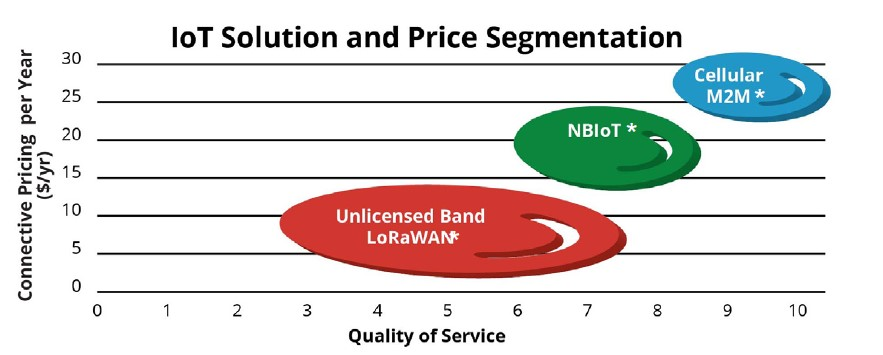
\includegraphics[width=\linewidth]{Assets/loracost.png}
	\caption{دسته‌بندی هزینه نگهداری سالیانه راهکارهای مختلف در حوزه اینترنت‌اشیاء.}
	\label{fig:loracost}
\end{figure}

2. طول عمر باتری و تاخیر در \متن‌لاتین{Downlink}: طول عمر باتری از دو جنبه مهم قابل بررسی است: \\
مصرف جریان تجهیزات (پیک و میانگین) و نقش پروتکل\متن‌لاتین{LoRaWAN}. یک پروتکل آسنکرون مبتنی بر \متن‌لاتین{ALOHA} می باشد، به این معنی که تجهیزات مادامی که درخواستی مطرح نشود می تواند استراحت کنند. در حالی‌که در پروتکل سنکرون مبتنی بر شبکه\متن‌لاتین{Cellular} ، تجهیزات می‌بایست به صورت منظم با شبکه هماهنگ شوند. به عنوان مثال به طور میانگین تلفن‌های سلولار می‌بایست هر 5/1 ثانیه با شبکه سینک شود حتی چنانچه استفاده نشوند. در مقایسه در \متن‌لاتین{NB-IOT} نیز اگرچه همزمانی اغلب کمتر اتفاق می‌افتد اما همچنان منظم می‌باشد که سبب می‌شود انرژی بیشتری از باتری استفاده نماید. در حالی که مدولاسیونی که در شبکه سلولار مورد استفاده قرار می‌گیرد از دیدگاه استفاده از طیف موثرترین است اما از دیدگاه تجهیزات انتهایی چندان کارآمد نیست. در مدولاسیون سلولار \متن‌لاتین{FDMA} به منظور ایجاد مدولاسیون به یک فرستنده خطی نیاز داریم و یک فرستنده خطی نیز در مقایسه با مدولاسیون غیر خطی به میزان بیشتر از پیک جریان نیاز دارد. این میزان جریان بالاتر از پیک، نیاز به باتری بیشتر و گرانتری دارد تا آن را پشتیبانی نماید. خاصیت سنکرون یک شبکه سلولار فواید بسیاری در کاربردهایی که نیاز به تاخیر کوتاه در \متن‌لاتین{downlink} دارند ایجاد می نماید.

\متن‌لاتین{NB-IOT} همچنین می‌تواند برای کاربردهایی که نیاز به \متن‌لاتین{throughput} داده بالاتری دارند نرخ داده بالاتری را ارائه نماید. \متن‌لاتین{LoRaWAN} با پشتیبانی از کلاس \متن‌لاتین{B} که به گونه ای طراحی شده است که تاخیر \متن‌لاتین{downlink} را با بیداری تجهیزات در فواصل قابل برنامه ریزی کاهش دهد. برای کاربردهایی با نیازمندی‌هایی همچون ارتباطات بسیار مکرر و تاخیر خیلی کوتاه یا حجم اطلاعات بالا، \متن‌لاتین{NB-IOT} بهترین گزینه خواهد بود. اگرچه در کاربردهایی که نیاز به باتری با طول عمر بسیار بالا و هزینه بهبود یافته می باشد، \متن‌لاتین{LoRa} بهترین گزینه است. در شکل \رجوع{fig:lorarange}، مقایسه‌ای بین رنج پوشش‌دهی، قیمت ماژول و طول عمر باتری را مشاهده می‌کنید.

\begin{figure}[!h]
	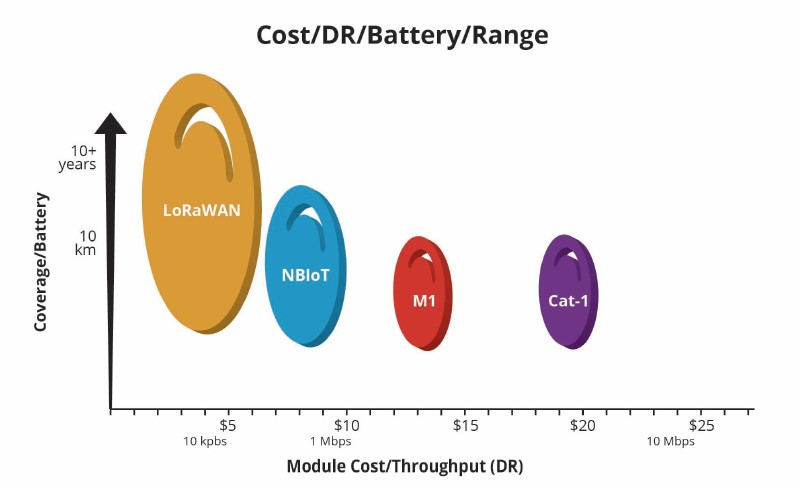
\includegraphics[width=\linewidth]{Assets/lorarange.png}
	\caption{مقایسه‌ای بین رنج پوشش‌دهی، قیمت ماژول و طول عمر باتری.}
	\label{fig:lorarange}
\end{figure}

3. پوشش شبکه: یکی از فواید \متن‌لاتین{NB-IOT} این است که زیر ساختهای موجود به منظور سرویس دهی، قابل ارتقا می‌باشد، اگرچه این ارتقا محدود به ایستگاه‌های پایه \متن‌لاتین{LTE}/\متن‌لاتین{4G} می‌باشد و گران است. البته این استراتژی برای محیط‌های شهری پرتراکم که پوشش شبکه \متن‌لاتین{LTE}/\متن‌لاتین{4G} دارند مناسب می‌باشد، برای نواحی روستایی و یا غیرشهری که چنین پوشش‌دهی وجود ندارد ایده آل نیست. ویژگی های \متن‌لاتین{NB-IOT} در ماه ژوئن سال 2016 منتشر شد و پیش‌بینی شد که در نیمه اول سال 2017 در دسترس باشد. یکی از ویژگی‌های \متن‌لاتین{LoRaWAN} قابلیت کار اجزای آن در مدل‌های اینترپرایز و خصوصی به خوبی مدلهای شبکه عمومی می‌باشد. در حالی که \متن‌لاتین{NB-IOT} تنها محدود به مدل عمومی ایستگاه‌های پایه سلولار می باشد.

4. هزینه تجهیزات و شبکه: از دیدگاه تجهیزات انتهایی، پروتکل \متن‌لاتین{LoRaWAN} در مقایسه با \متن‌لاتین{NB-IOT} ساده‌تر است و به آسانی با هزینه پایین قابل پیاده سازی است. همچنین مدولاسیون و پروتکل \متن‌لاتین{NB-IOT} پیچیده‌تر است. بنابراین هزینه راهکار را افزایش می‌دهد.

\قسمت{معماری \متن‌لاتین{LoRa}}
\متن‌لاتین{LoRa} مخفف \متن‌لاتین{Long Range Ratio} است و یک فناوری مدولاسیون طیف گسترده\پانویس{ Spread Spectrum} است که از فناوری CSS\پانویس{Chirp Spread Spectrum} برگرفته شده است. CSS در سال 1940 برای رادارهای نظامی طراحی شد. مهم‌ترین ویژگی‌های \متن‌لاتین{LoRa} برد بالا، هزینه پیاده‌سازی پایین، مصرف توان پایین و سرعت انتقال داده پایین می‌باشدکه کاربرد‌های متنوعی در حوزه اینترنت اشیاء دارد. در \متن‌لاتین{LoRa}، گسترش طیف با تولید یک سیگنال \متن‌لاتین{CHIRP} که بطور مداوم در فرکانس‌های مختلف جابجا می‌شود. این فناوری، در ابتدا در شهر گرنوبل فرانسه توسط شرکت \متن‌لاتین{SEMTECH} در سال 2012 معرفی شد. شرکت \متن‌لاتین{SIMTECH} لایسنس محصولات خود را به‌عنوان \متن‌لاتین{IP CORE} به فروش می‌رساند و شرکت‌های دیگر از جمله \متن‌لاتین{MICROCHIP}، \متن‌لاتین{NXP} و \متن‌لاتین{AI-THINKER} ماژول خود را بر اساس طراحی‌های شرکت \متن‌لاتین{SIMTECH} می‌سازند.

در بازار ایران تنها محصولات شرکت \متن‌لاتین{AI-THINKER} در دو مدل \متن‌لاتین{RA-01} و \متن‌لاتین{RA-02} عرضه می‌شود که هر دو بر اساس معماری \متن‌لاتین{SX1278} شرکت \متن‌لاتین{SEMTECH} ساخته شده‌اند. هسته پردازنده این ماژول از محصولات شرکت STM است که ما برای این پروژه از مدل \متن‌لاتین{RA-02} استفاده کردیم که علاوه پروتکل \متن‌لاتین{LoRa}، پروتکل‌های FSK و OOK را نیز پشتیبانی می‌کند. در شکل \رجوع{fig:loraRA02} نمای داخلی و خارجی این ماژول را مشاهده می‌کنید.

\begin{figure}[H]
	\begin{subfigure}[b]{0.5\textwidth}
		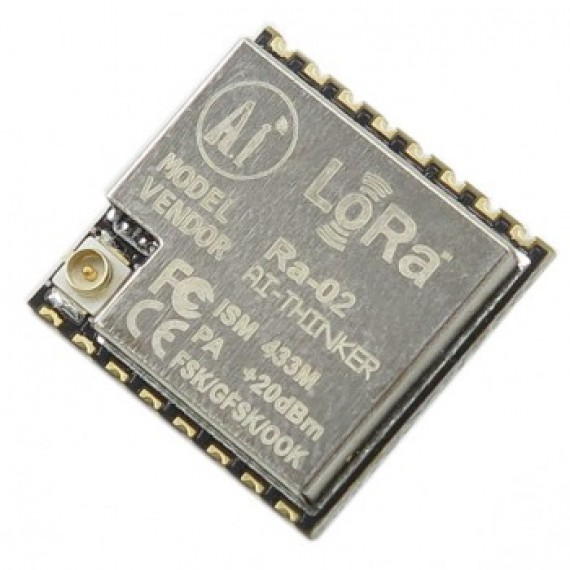
\includegraphics[width=\linewidth]{Assets/loraouter.png}
		\caption{نمای خارجی ماژول \متن‌لاتین{RA-02}}
		\label{fig:loraouter}
	\end{subfigure}
	\begin{subfigure}[b]{0.5\textwidth}
		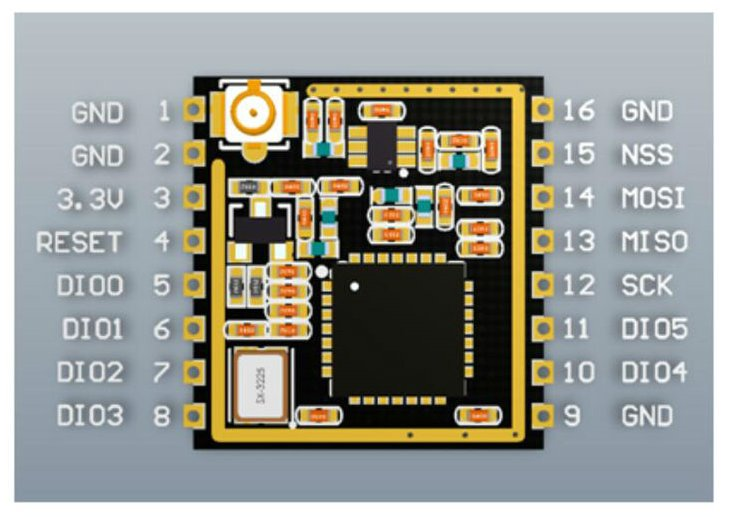
\includegraphics[width=\linewidth]{Assets/lorainner.png}
		\caption{نمای داخلی ماژول \متن‌لاتین{RA-02}}
		\label{fig:lorainner}
	\end{subfigure}
	\caption{نمای داخلی و خارجی ماژول \متن‌لاتین{RA-02}.}
	\label{fig:loraRA02}
\end{figure}

ماژول‌های \متن‌لاتین{LoRa} در بازه‌های فرکانسی مختلف تولید می‌شود. ماژول خریداری شده حتما می‌بایست با قوانین سازمان تنظیم مقررات و ارتباطات رادیویی کشور مورد نظر، سازگاری داشته باشد. (در آسیا، فرکانس 433MHZ، در اروپا 868MHZ و در آمریکای شمالی 915MHZ محدوده مجاز است)

در ژانویه سال 2018، نسل جدیدی از \متن‌لاتین{LoRa} رونمایی شد که از ویژگی‌های آن، افزایش توان انتقال، کاهش توان مصرفی و کاهش ابعاد آن نسبت به مدل‌های قدیمی است. البته هنوز محصولی از آن به بازار عرضه نشده است.

نرخ انتقال داده: حداکثر نرخ داده در \متن‌لاتین{LoRa}  مقدار 30kb/s می‌باشد که نسبتا مقدار کمی است.

\متن‌لاتین{CSS} (\متن‌لاتین{Chirp Spread Spectrum}): یک \متن‌لاتین{Chirp}، یک سیگنال سینوسی از افزایش یا کاهش فرکانس است که به ماهیت سیگنال‌های \متن‌لاتین{Chirp} برای پخش طیف پهنای‌باند سیگنال ارسالی وابسته است. یک \متن‌لاتین{Chirp} از افزایش فرکانس را که \متن‌لاتین{up-chirp} می‌نامند، در شکل \رجوع{fig:upchrip} مشاهده می‌کنید.

\begin{figure}[!h]
	\centering
	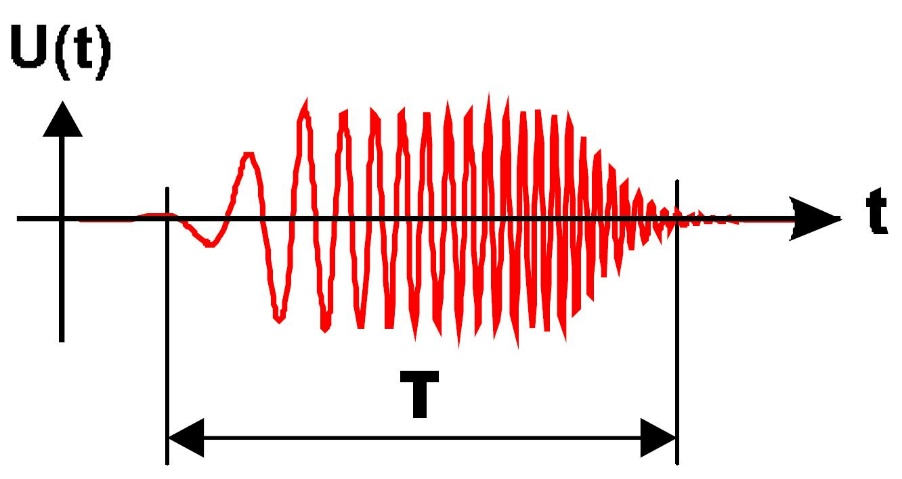
\includegraphics[width=0.7\linewidth]{Assets/upchrip.png}
	\caption{\متن‌لاتین{up-chirp} در واحد زمان.}
	\label{fig:upchrip}
\end{figure}

‌‌‌‌‌یک \متن‌لاتین{Chirp} از کاهش فرکانس را که \متن‌لاتین{down-chirp} می‌نامند، در شکل \رجوع{fig:downchrip} مشاهده می‌کنید.

\begin{figure}[!h]
	\centering
	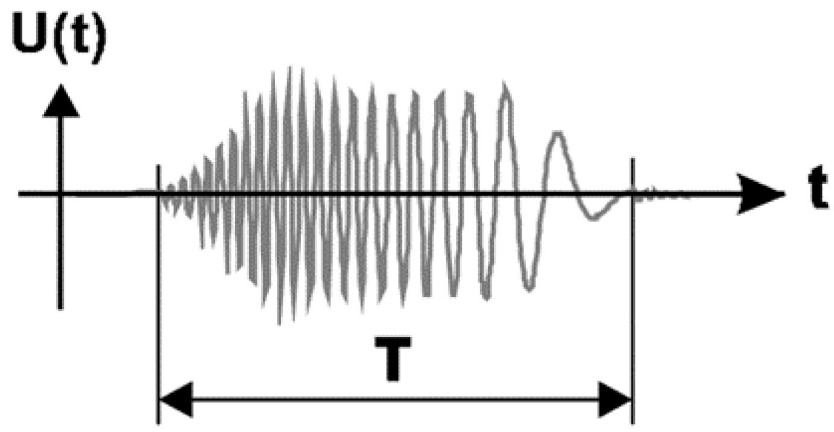
\includegraphics[width=0.7\linewidth]{Assets/downchrip.png}
	\caption{ \متن‌لاتین{down-chirp} در واحد زمان.}
	\label{fig:downchrip}
\end{figure}

\متن‌لاتین{up-chirp} دارای مقدار مثبت و \متن‌لاتین{down-chirp} دارای مقدار منفی است. تغییر فرکانس می‌تواند خطی یا نمایی باشد. پهنای باند سیگنال \متن‌لاتین{Chirp}، تفاومت بین فرکانس شروع و فرکانس پایانی است.
1. فشرده‌سازی پالس: فشرده‌سازی پالس، فرآیندی است که طی آن پالس طولانی مدت با قدرت پیک پایین به یک پالس کوتاه‌مدت با پیک بالا  تبدیل می‌شود. پالس‌های مستقیم با استفاده از یک فیلتر همگام\پانویس{matched filter} و توسط هم‌بستگی\پانویس{correlation}، فشرده‌سازی می‌شوند. شکل \رجوع{fig:CSS} ساختمان سیستم \متن‌لاتین{CSS} را نشان می‌دهد داده‌ها با استفاده از \متن‌لاتین{up-chirp} و \متن‌لاتین{down-chirp} در سمت فرستنده مدوله می‌شود و با استفاده از همبستگی با فیلتر همگرا برای فشرده‌سازی پالس، به‌دست می‌آیند و به‌عنوان پالس تیز انرژی بالا که می‌تواند به راحتی رمزگشایی شود.

\begin{figure}[!h]
	\centering
	\includegraphics[width=\linewidth]{Assets/CSS.png}
	\caption{نمودار بلوک \متن‌لاتین{CSS}.}
	\label{fig:CSS}
\end{figure}

یکی از مهم‌ترین ویژگی‌های \متن‌لاتین{CSS}، مقیاس‌پذیری نرخ سرعت داده است. برای گسترش سیگنال هر دو در زمان و فرکانس به‌طور مستقل، می‌توان از طیف گسترده‌ای از \متن‌لاتین{Chirp} استفاده  کرد.

2. پخش فرکانسی: همانطور که در بخش قبلی توضیح داده شده است، گسترش پهنای‌باند سیگنال می‌تواند در کاهش اثر نویز کانال کمک کند و سیگنال را در برابر تداخل ایمن سازد. با استفاده از پالس‌های \متن‌لاتین{Chirp} پهنای‌باند بسیار بالاتر، پهنای باند سیگنال می‌تواند به اندازه مورد نیاز افزایش یابد.

3. پخش زمانی: از آنجایی که پهنای‌باند سیگنال‌های \متن‌لاتین{Chirp} تنها به شروع و پایان فرکانس \متن‌لاتین{Chirp} بستگی دارد، سرعت داده از مدولاسیون \متن‌لاتین{Chirp} می‌تواند به طور مستقل از پهنای باند بالا و پایین‌ شود. بنابراین این امکان وجود دارد که آزادانه پهنای‌باند و سرعت داده انتخاب شود.

ساختمان بسته\پانویس{Packet} \متن‌لاتین{LoRa}: ساختمان بسته \متن‌لاتین{LoRa} را در شکل \رجوع{fig:lorapacket} مشاهده می‌کنید.

\begin{figure}[!h]
	\centering
	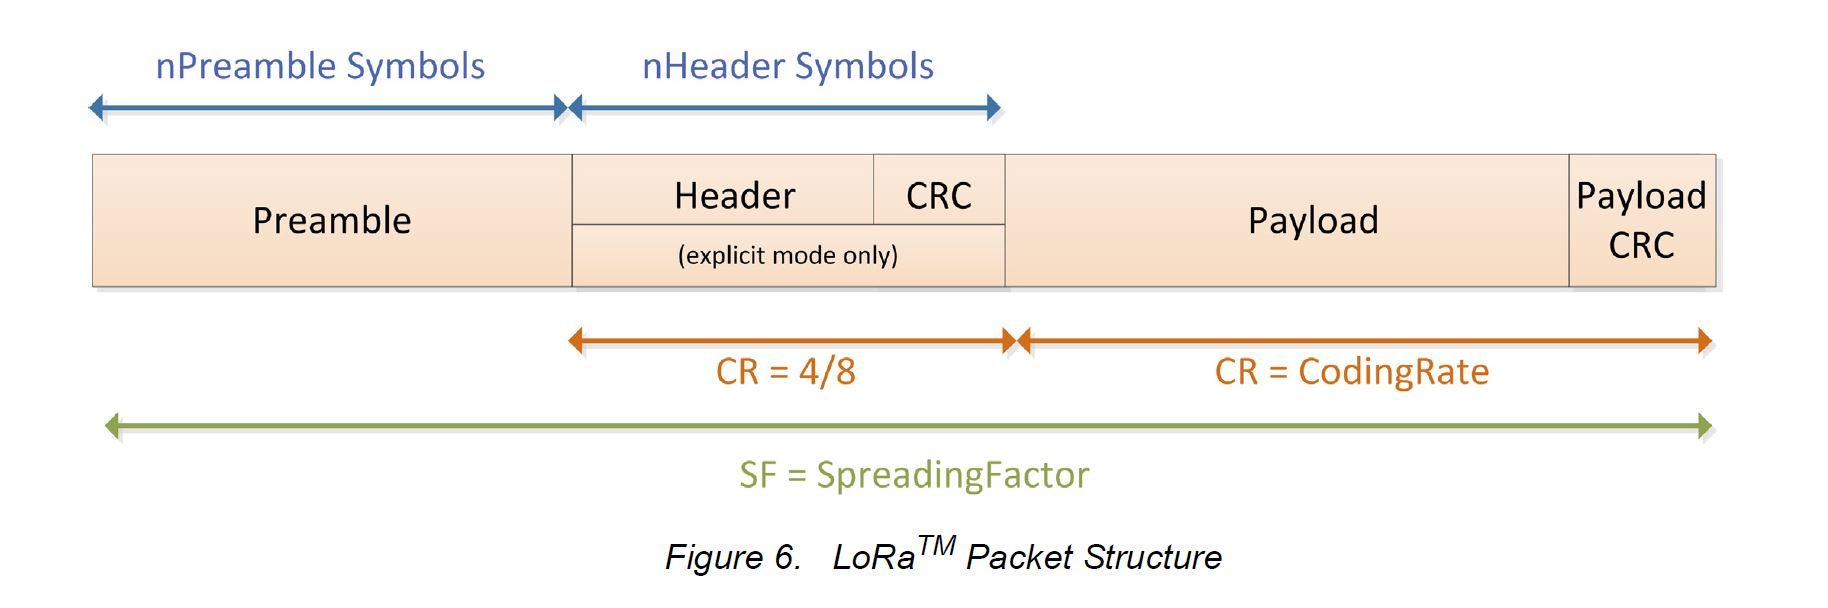
\includegraphics[width=\linewidth]{Assets/lorapacket.png}
	\caption{ساختمان بسته \متن‌لاتین{LoRa}.}
	\label{fig:lorapacket}
\end{figure}
\noindent
به‌طورکلی در \متن‌لاتین{LoRa} دو فرم برای ارسال داده داریم و می‌توان آن را با بیت \متن‌لاتین{ImplicitHeaderModeOn} که در رجیستر \متن‌لاتین{RegModemConfig1} وجود دارد، تنظیم کرد:

1. \متن‌لاتین{Explicit}: شامل یک سرصفحه\پانویس{Header} که حاوی اطلاعات در مورد تعداد بایت‌ها، نرخ کدگذاری و وجود یا عدم وجود \پانوشت{نام واحدی است مشخص‌کردن خطای داده ارسالی که گیرنده می‌تواند به کمک آن سرصفحه‌های نامعتبر را دریافت نکند.} 16 بیتی در بسته. در این مدل، حضور \متن‌لاتین{CRC} در انتهای بارگیری تنها در سمت فرستنده از طریق بیت \متن‌لاتین{RxPayloadCrcOn} در رجیستر \متن‌لاتین{RegModemConfig1} ثبت می‌شود. در سمت گیرنده، این بیت استفاده نمی‌شود و فقط بارگیری دریافت می‌شو. کاربر می‌بایست بیت \متن‌لاتین{CrcOnPayload} در رجیستر \متن‌لاتین{RegHopChannel} را کنترل کند.در صورت ‘1’ بودن باید بیت \متن‌لاتین{IrqFlag} را از رجیستر \متن‌لاتین{PayloadCrcError} تا مطمئن شود که \متن‌لاتین{CRC} معتبر است. ‘0’ بودن بیت \متن‌لاتین{CrcOnPayload}، به این معنی است که \متن‌لاتین{CRC} در بارگیری حضور ندارد. در نتیجه \متن‌لاتین{IrqFlag} حتی اگربارگیری خطا داشته باشد، فعال نخواهد شد. به جدول \رجوع{table:ExplicitCRC} توجه کنید.


\begin{table}[!h]
	\centering
	\caption{وضعیت CRC در حالت \متن‌لاتین{Explicit} .}
	\label{table:ExplicitCRC}
	\begin{latin}
		\begin{tabular}{|c|c|c|c|}
			\hline
			\متن‌لاتین{Explicit Header} & \متن‌لاتین{Transmitter} & \متن‌لاتین{Receiver} & \متن‌لاتین{CRC Status}\\
			\hline
			\multirow{4}{7em}{\متن‌لاتین{Value of the bit RxPayloadCrcOn}} & 0 & 0 & \متن‌لاتین{CRS is not checked}\\
			&	0 & 1 & \متن‌لاتین{CRS is not checked}\\
			&	1 & 0 & \متن‌لاتین{CRS is checked}\\
			&	1 & 1 & \متن‌لاتین{CRS is checked}\\
			\hline
		\end{tabular}
	\end{latin}
\end{table}


2. \متن‌لاتین{Implicit}: 
در جایی که مقدار بارگیری\پانویس{Payload}، نرخ کدگذاری و حضور \متن‌لاتین{CRC} ثابت یا شناخته شده است بهتر است سر صفحه را از بسته حذف کنیم و این مقادیر را دستی تنظیم کنیم. در این مدل لازم‌است تا بیت \متن‌لاتین{RxPayloadCrcOn} در رجیستر \متن‌لاتین{RegModemConfig1} را در هر دو سمت فرستنده و گیرنده تنظیم کنیم. توجه داشته باشید که اگر مقدار پارامتر SF برابر 6 باشد، ماژول فقط در مدل \متن‌لاتین{Implicit} می‌تواند کار کند. 

پیشوند\پانویس{Preamble}: این قسمت برای همگام‌سازی گیرنده با داده ورودی کاربرد دارد. بطور پیش‌فرض، بسته با دنباله‌ای به طول پیوند 12نمادی\پانویس{Symbol} پیکربندی می‌شود.این مقدار با تنظیم رجیستر \متن‌لاتین{PreambleLenght} قابل برنامه‌ریزی است و میتواند بین 6 تا 65535 مقدار بگیرد. این رجیستر باید در سمت فرستنده و گیرنده باید یکسان پیکربندی شود. در جایی که طول پیوند فرستنده متغیر است، در گیرنده باید بیشترین طول پیوند که ممکن‌است رخ دهد، تنظیم شود.

نرخ کد‌گذاری: جهت بهبود پایداری اتصال، از این ویژگی برای اصلاح خطاهای پیش‌رو استفاده می‌شود. اضافه کردن این ویژگی به کد، موجب افزایش تعداد بیت‌های ارسالی می‌شود. در جدول1 نرخ \متن‌لاتین{OVERHEAD} به ازاء نرخ کدگذاریهای مختلف نشان داده شده است.

عامل گسترش\پانویس{Spreading Factor (SF)}: پارامتری است که‌ مقدار آن می‌تواند بین 6 تا 12 باشد. هر چه مقدار آن بیشتر باشد، نرخ دیتا پایین‌تر، حساسیت، برد و توان مصرفی آن بیشتر می‌شود و هرچه مقدار آن پایین‌تر باشد، نرخ دیتا بالاتر، حساسیت، برد و توان مصرفی آن کمتر می‌شود. همچنین با فرکانس و پهنای باند مشخص، اگر عامل‌گسترش فرستنده با گیرنده یکسان نباشد، گیرنده نمی‌تواند پیام را دریافت کند. در جدول \رجوع{table:SFSNR} \متن‌لاتین{SF}های مختلف و پارامتر \متن‌لاتین{SNR} آن‌ها را نمایش می‌دهد. در جدول \رجوع{table:lorabitrate} نرخ داده و \متن‌لاتین{SF}های مختلف را نمایش می‌دهد.

\begin{table}[!h]
	\centering
	\caption{مقدار \متن‌لاتین{SNR} به ازاء عامل گسترش‌های مختلف.}
	\label{table:SFSNR}
	\begin{latin}
		\begin{tabular}{|C{3.5cm}|C{3.5cm}|C{3.5cm}|}
			\hline
			\متن‌لاتین{Spreading Factor (RegModulationCfG)} & \متن‌لاتین{Spreading Factor  (Chips / symbol)} & \متن‌لاتین{LoRa Demodulator SNR (dB)} \\			
			\hline
			6 & 64 & -5\\
			7 & 128 & -7٫5\\
			8 & 256 & -10\\
			9 & 512& -12٫5\\
			10 & 1024 & -15\\
			11 & 2048 & -17٫5\\
			12 & 4096 & -20\\
			\hline
		\end{tabular}
	\end{latin}
\end{table}

\begin{table}[!h]
	\centering
	\caption{نرخ داده‌های  \متن‌لاتین{LoRa}.}
	\label{table:lorabitrate}
	\begin{latin}
		\begin{tabular}{|C{3cm}|C{3cm}|}
			\hline
			\متن‌لاتین{Spreading Factor} & \متن‌لاتین{Bit rate (bits / s)} \\			
			\hline
			7 & 5469 \\
			8 & 3125 \\
			9 & 1758 \\
			10 & 977 \\
			11 & 537 \\
			12 & 293 \\
			\hline
		\end{tabular}
	\end{latin}
\end{table}

\متن‌لاتین{Time-On-Air}: مدت زمانی که طول می‌کشد تا یک بسته از ماژول فرستنده به ماژول گیرنده برسد و مقدار آن از رابطه زیر بدست می‌آید:									
\begin{equation}
	T_s=\frac{2^{SF}}{BW}
\end{equation}		
\noindent
پارامترهای مختلفی از جمله نرخ کدگذاری، پهنای باند، \متن‌لاتین{SF}،  جهت رسیدن به برد و سرعت داده مورد استفاده قرار می‌گیرند. در جدول تصویر \رجوع{}fig:TOA مقدار \متن‌لاتین{TOA} را با ترکیب مقادیر مختلف این پارامترها و نیز سایز بارگیری‌های مختلف نشان داده شده است.

\begin{figure}[!h]
	\centering
	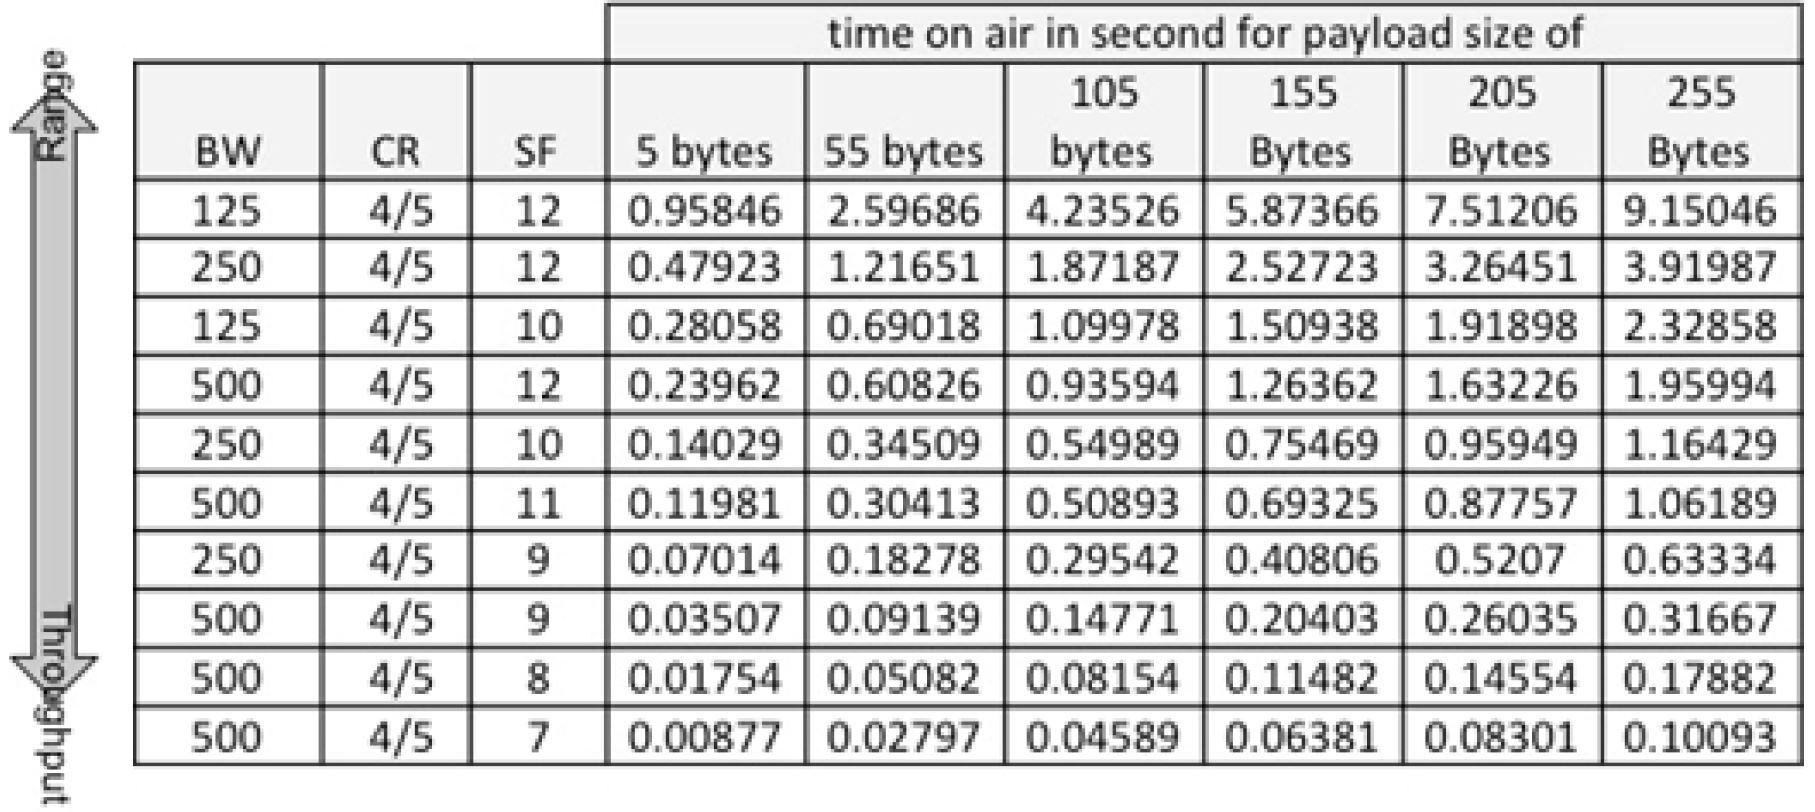
\includegraphics[width=\linewidth]{Assets/TOA.png}
	\caption{مقدار \متن‌لاتین{TOA} در برای ترکیب‌های مختلف تنظیمات \متن‌لاتین{LoRa}.}
	\label{fig:TOA}
\end{figure}

نحوه پیکربندی رجیسترهای درون ماژول \متن‌لاتین{LoRa}: این کار می‌بایست از طریق پروتکل \متن‌لاتین{SPI} انجام شود. نوشتن رجیسترها تنها در \متن‌لاتین{Sleep Mode} امکان‌پذیر است. (مد کاری ماژول درون رجیستر \متن‌لاتین{RegOpMode} پیکربندی می‌شود.)

\قسمت{انواع پیاده‌سازی}

\زیرقسمت{پیاده‌سازی \متن‌لاتین{LoRa}}
در این روش تعدادی ماژول \متن‌لاتین{LoRa} به صورت خصوصی با هم ارتباط دارند. پروژه مربوطه نیز بر اساس همین روش پیاده‌سازی شده است.

\زیرقسمت{\متن‌لاتین{LoRaWAN}}

\begin{figure}[!h]
	\centering
	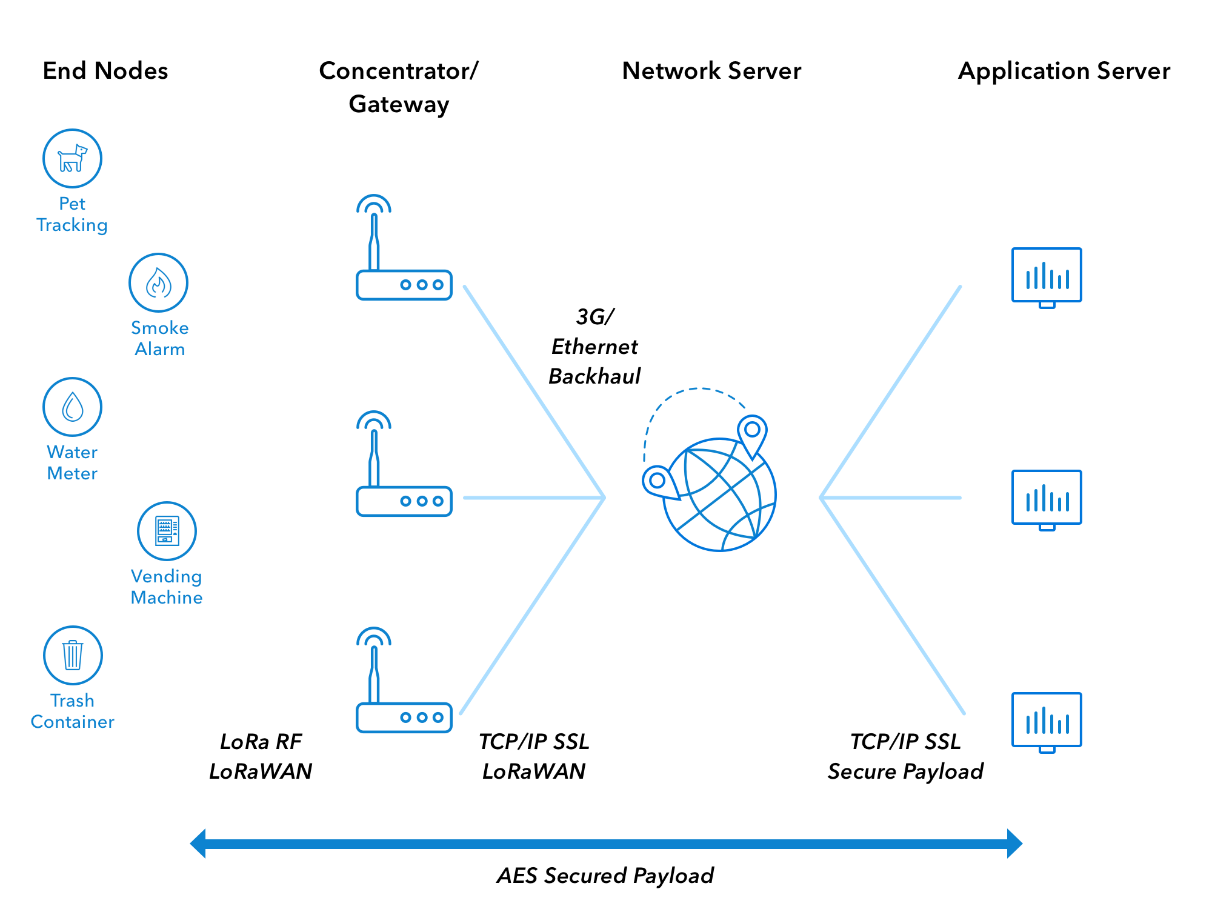
\includegraphics[width=\linewidth]{Assets/lorawan.png}
	\caption{ نمونه ای از شبکه \متن‌لاتین{LoRaWAN}.}
	\label{fig:LoRaWAN}
\end{figure}

همانطور که در شکل \رجوع{fig:LoRaWAN} مشاهده می‌کنید، معماری شبکه \متن‌لاتین{LoRaWAN} به صورت توپولوژی ستاره یا استار میباشد که در آن دروازه‌ها پیام‌ها را بین دستگاه‌های پایانی و سرور مرکزی شبکه انتقال می‌دهند. دروازه‌ها مانند یک پل نامرئی عمل می‌کنند و از طریق اتصالات استاندارد آی‌پی به سرور در شبکه متصل می‌شوند، به سادگی بسته‌های \متن‌لاتین{RF} را به بسته‌های \متن‌لاتین{IP} تبدیل می‌کنند و بالعکس. ارتباطات بی‌سیم از مزایای برد زیاد لایه‌فیزیکی \متن‌لاتین{LoRa} بهره می‌برد و اجازه می‌دهد یک لینک تک کانون بین دستگاه پایانی و یا یک یا چند دروازه باشد. تمام حالت ها قادر به برقراری ارتباط دو طرفه هستند و پشتیبانی از گروه‌های آدرس‌دهی چندرسانه‌ای برای استفاده کارآمد از طیف در حین انجام وظایف مانند ارتقاء نرم‌افزار ها مانند \متن‌لاتین{Firmware} (\متن‌لاتین{FOTA}) یا سایر پیام‌های اپگرید وجود دارد. این شیوه پیاده سازی در اصطلاح، \متن‌لاتین{LoRaWAN} نامیده می‌شود. همچنین در این نوع پیاده‌سازی می‌توان از ماژول \متن‌لاتین{LoRa} به‌عنوان موقعیت‌یاب (بدون استفاده از \متن‌لاتین{GPS}) استفاده کرد. به این صورت که تاخیر دریافت پیام توسط دروازه‌های اطراف ماژول سنجیده می‌شود و بر اساس الگوریتم خاص، موقعیت جغرافیایی ماژول به‌دست می‌آید.

اتحادیه \متن‌لاتین{LoRa}1، در سال 2015 برای پشتیبانی از پروتکل \متن‌لاتین{LoRaWAN} تشکیل شده است. این اتحادیه، بیش از 500 عضو دارد که مهم ترین آنها، \متن‌لاتین{IBM}, \متن‌لاتین{ACTILITY}, \متن‌لاتین{MICROCHIP}, \متن‌لاتین{ORANGE}, \متن‌لاتین{CISCO}, \متن‌لاتین{KPN}, \متن‌لاتین{SWISSCOM}, \متن‌لاتین{SIMTECH}, \متن‌لاتین{BOUYGUES}, \متن‌لاتین{TELECOM}, \متن‌لاتین{SINGTEL}, \متن‌لاتین{PROXIMUS} می‌باشند.

گیتوی‌ها هم می‌تواند خودش سرور باشد و هم می‌تواند بعنوان \متن‌لاتین{Packet Forwarder} عمل کند و دیتا را به سروری مانند TTN2 که دارای پلتفرمی \متن‌لاتین{user friendly} است، ارسال کند. برای این‌کار، ابتدا در سایت ثبت نام می‌کنیم و پس از ورود به اکانت خود، گیتوی مورد نظر را رجیستر می‌کنیم. از بخش  \متن‌لاتین{CONSOLE} -> \متن‌لاتین{GATEWAYS} -> \متن‌لاتین{register gateway} صفحه‌ای همانند شکل \رجوع{fig:TTNregister} ظاهر می‌شود.

\begin{figure}[!h]
	\centering
	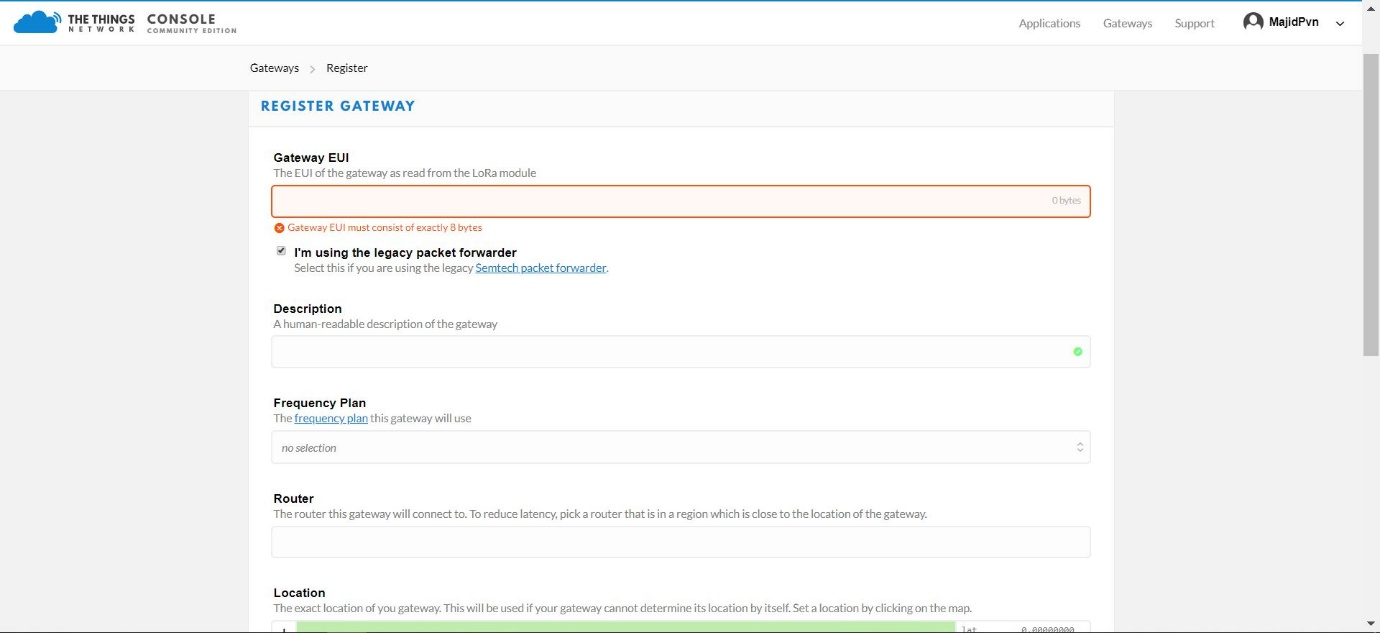
\includegraphics[width=\linewidth]{Assets/TTNregister.png}
	\caption{فرم رجیستر گیتوی در سایت \متن‌لاتین{TTN}.}
	\label{fig:TTNregister}
\end{figure}
 
در اینجا باید تیک \متن‌لاتین{legacy packet forwarder} را بزنیم و یک ایدی منحصر به فرد دلخواه وارد کنیم. قسمت بعدی مربوط به توضیحات است که می‌توان توضیحی از وضعیت، مدل یا هر اطلاعاتی که در مورد ها مورد نیاز است را وارد می‌کنیم. (این فیلد میتواند خالی باشد.). نمونه‌هایی از گیتوی‌ها را در شکل \رجوع{fig:lorawangateway} مشاهده می‌کنید.

\begin{figure}[!h]
	\centering
	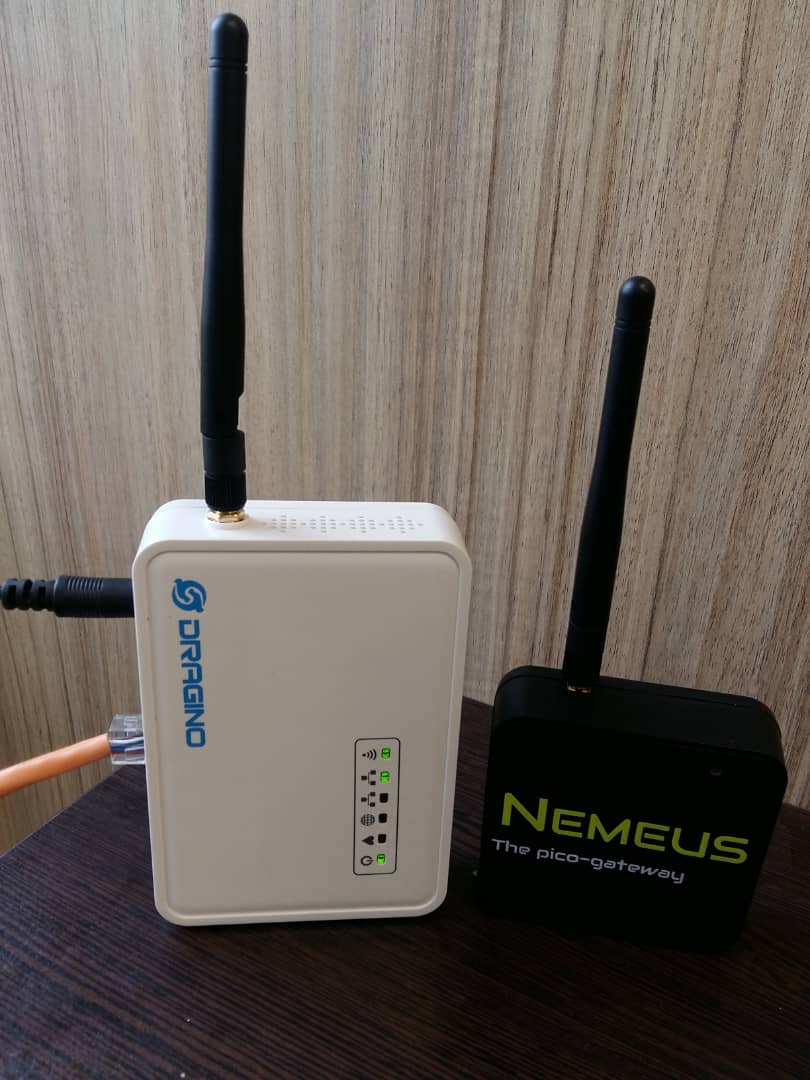
\includegraphics[width=\linewidth]{Assets/lorawangateway.png}
	\caption{دو نمونه از گیتوی‌ها با پشتیبانی از \متن‌لاتین{LoRaWAN}.}
	\label{fig:lorawangateway}
\end{figure}

گیتوی سمت راستی یک گیتوی معمولی و نسبتا ارزان‌تری است اما گیتوی سمت چپی امکانات بیشتری دارد که در ادامه توضیح مختصری درباره آن خواهیم داد.

گیتوی \متن‌لاتین{DRAGINO-LG01}: شرکت \متن‌لاتین{DRAGINO}، یک شرکت فعال در کشور چین است که بر روی اینترنت اشیاء متمرکز است. این مدل می‌تواند بعنوان مودم اینترنت عمل کند. یعنی کابل شبکه به آن متصل شود و اینترنت را از طریق \متن‌لاتین{WIFI} در محیط پخش کند. همچنین می‌توان به‌عنوان گیتوی \متن‌لاتین{LoRaWAN} از آن استفاده کرد. بخشی از مدار داخلی آن از یک ماژول \متن‌لاتین{RFM95} شرکت \متن‌لاتین{MICROCHIP} و یک میکروکنترلر \متن‌لاتین{ATMEGA328} تشکیل شده است که کاربر می‌تواند برنامه موردنظر خود را در محیط آردینو\پانویس{Arduino} بنویسد و درون میکروکنترلر آپلود کند. روش آپلود فایل هم به دو صورت است هم می‌توان از پلتفرم داخلی آن فایل HEX را آپلود کرد و هم می‌توان از محیط آردوینو این کار را انجام دهد. لازم به ذکر است که این مدل فقط از کلاس‌های A و C پشتیبانی می‌کند.

\زیرقسمت{انواع کلاس در شبکه \متن‌لاتین{LoRaWAN}}
         
1. کلاس A: کمترین توان، دستگاه‌های پایانی دو طرفه:
کلاس پیش‌فرض باید توسط تمام \متن‌لاتین{Node}\پانوشت{همان \متن‌لاتین{End-Device} است که دیتا را از نقاط مختلف به گیتوی ارسال می‌کند.}ها پشتیبانی شود. ارتباط کلاس A همیشه توسط دستگاه پایانی آغاز می شود و کاملا ناهمگام است. هر گونه انتقال uplink\پانوشت{انتقال دیتا از \متن‌لاتین{NODE} به اپلیکیشن سرور} می‌تواند در هر زمانی ارسال شود و همچنین توسط دو downlink\پانوشت{انتقال پیام از اپلیکیشن سرور به \متن‌لاتین{NODE}} کوتاه دنبال می‌شود.

\متن‌لاتین{Node} ها این قابلیت را دارا خواند بود که توسط برنامه مشخص شده خود وارد حالت خواب بشوند. در حالت خواب با کم شدن قدرت مصرف دستگاه به حداقل میرسد و به همین علت هست که یک باتری برای دستگاه یک یا چند سال کار میکند. همچنین در این حالت دیگر نیازی به شبکه برای بیداری دوره ای دستگاه وجود ندارد. همین علت است که کلاس A کمترین مصرف را در این کلاس بندی پروتکل دارد. در این کلاس هر موقع که ارتباطی برقرار شود اجازه برقراری آن ارتباط به آن داده میشود. از آنجا که ارتباط \متن‌لاتین{downlink} همیشه باید به یک انتقال \متن‌لاتین{uplink} با برنامه ای که توسط برنامه نهایی دستگاه تعریف می شود پیروی می کند،اگر ارتباط \متن‌لاتین{downlink} بعدی بیاید باید در سرور شبکه نگهداری شود تا کار پیام قبلی تمام شود.

2. کلاس B – دستگاه های پایانی دو طرفه با تاخیر قطعی \متن‌لاتین{Downlink}:
علاوه بر کلاس A ، دستگاه ها در کلاس B با استفاده از موج‌های دوره‌ای، همگام با شبکه می‌شوند و در زمان‌های برنامه‌ریزی شده بازه پینگ های ‌\متن‌لاتین{downlink} را باز می کنند. با استفاده از این مورد شبکه توانایی ارسال ارتباطات ‌\متن‌لاتین{downlink} را با تاخیر قطعی بدست می آورد، اما همین امر باعث افزایش مصرف انرژی دستگاه پایانی میشود. زمان تاخیر تا ۱۲۸ ثانیه قابل برنامه ریزی است تا با برنامه های مختلف متفاوت باشد، و مصرف انرژی اضافی به اندازه کافی کم است که هنوز هم برای استفاده از باتری برای برنامه ها قابل اعتماد باشد.
3. کلاس C – کمترین زمان تاخیر، دستگاههای پایانی دو طرفه:
علاوه بر ساختار کلاس A که از ‌\متن‌لاتین{uplink} به دنبال دو مسیر ‌\متن‌لاتین{downlink} میباشد، کلاس C باعث کاهش زمان تأخیر در ‌\متن‌لاتین{downlink} می شود. چطور؟!!! با نگه داشتن \متن‌لاتین{Node} در تمام زمان هایی که دستگاه چیزی انتقال نمی دهد (نیمه دو طرفه). بر اساس این، سرور شبکه می تواند در هر زمان بر اساس فرضیه گیرنده دستگاه پایانی باز شود، بنابراین هیچ تأخیری نمی تواند یک انتقال ‌\متن‌لاتین{downlink} را شروع کند. کلاس C مناسب برای برنامه های کاربردی است که نیاز به قدرت و مصرف مداوم دارند. برای دستگاه هایی که از باتری استفاده می‌کنند، حالت تعویض موقت بین کلاس A و کلاس C امکان پذیر است و برای انجام وظایف متناوب مانند به روز رسانی سیستم‌عامل از طریق راه دور (\متن‌لاتین{OTA}\پانوشت{\متن‌لاتین{ OTA=Over The Air} به طور خلاصه به معنی بروزرسانی دستگاه ها از طریق اینترنت یا موارد دیگر از طریق فواصل دور است.}) مناسب است.

\قسمت{امنیت}

شبکه \متن‌لاتین{LoRaWAN} با تعدادی کلیدواژه امنیتی ارتباط برقرار می‌کند که طول تمامی آن‌ها 128بیت می‌باشند.

\متن‌لاتین{Network Session Key} (\متن‌لاتین{NwkSKey}): برای ارتباط میان \متن‌لاتین{Node} و سرور می‌باشد. این کلیدواژه، برای اعتبارسنجی پیام‌ها کاربرد دارد.

\متن‌لاتین{Application Session Key} (\متن‌لاتین{AppSKey}): این کلیدواژه جهت کدگذاری و دیکود کردن دیتای ارسالی (دریافتی) می‌باشد. به این صورت که کلیدواژه ای دلخواه خودمان در سمت \متن‌لاتین{Node} وارد می‌کنیم و با این کلیدواژه، دیتای ارسالی کدگذاری می‌شود و در سمت سرور تنها با وارد کردن همان کلیدواژه قادر به دیکود کردن آن می‌باشیم. این بدان معنی است که هیچ‌کسی غیر از خودتان قادر به دسترسی به دیتای ارسالی نخواهد داشت.

هر دو کلیدواژه‌های بالا برای هر دستگاهی منحصر به فرد است. اگر بخواهید این کلیدواژه‌ها را از راه دور و به‌طور دینامیکی تغییر دهید، باید از مد \متن‌لاتین{OTAA} استفاده کنید و اگر بخواهیم در هنگام ساخت دستگاه این اطلاعات را وارد کنیم و از راه دور امکان به تغییر آن وجود نداشته باشد، باید از مد \متن‌لاتین{ABP} استفاده کنیم.

\قسمت{ماژول \متن‌لاتین{RN2483}}
\begin{figure}[!h]
	\centering
	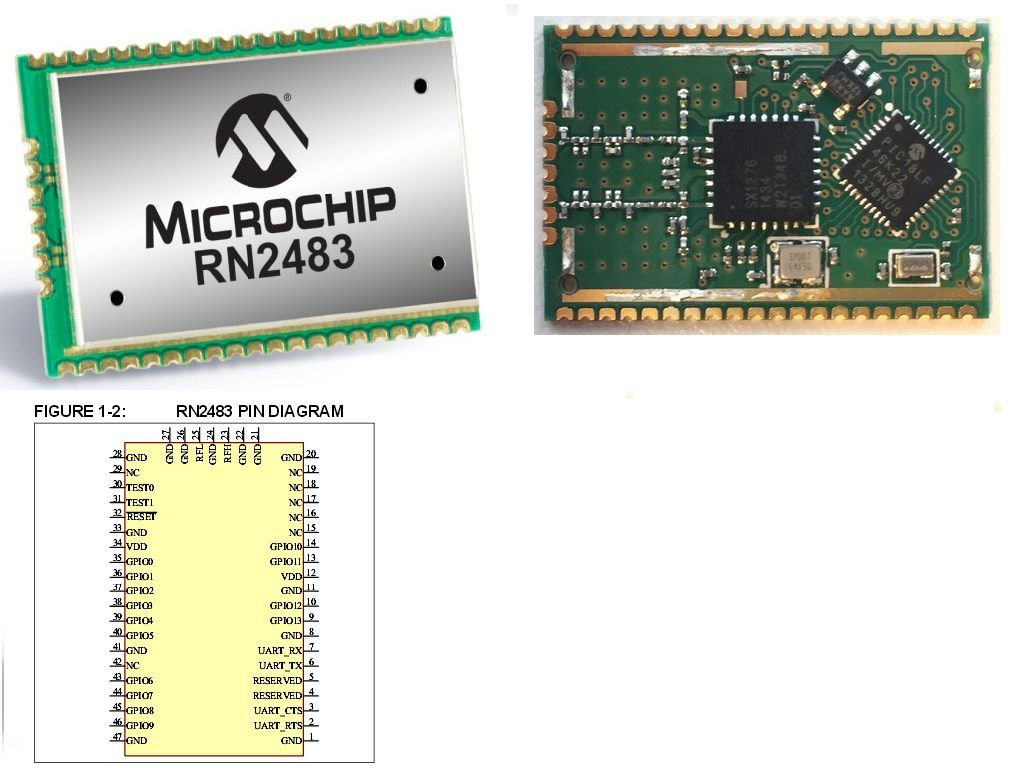
\includegraphics[width=\linewidth]{Assets/RN2483.png}
	\caption{نمای بیرونی، مدار داخلی و پایه‌های خروجی ماژول \متن‌لاتین{RN2483}.}
	\label{fig:RN2483}
\end{figure}
این ماژول متعلق به شرکت \متن‌لاتین{MICROCHIP} می‌باشد. همانطور که در شکل \رجوع{fig:RN2483} مشاهده می‌کنید، مدار داخلی آن از یک چیپ \متن‌لاتین{SX1276} شرکت \متن‌لاتین{SEMTECH} و یک میکروکنترلر \متن‌لاتین{PIC18LF} تشکیل شده است. و دارای دو خروجی آنتن با فرکانس‌های 433 مگاهرتز و 868 مگاهرتز می‌باشد که بسته به نیاز کاربر، می‌توان از یکی از آن‌ها استفاده کند. که این دو از طریق پروتکل \متن‌لاتین{SPI} باهم در ارتباط هستند و تعدادی کامند برای میکروکنترلر اش تعریف شده است که کاربر می‌تواند از طریق آن کامندها توسط پروتکل \متن‌لاتین{UART} با باد ریت 57600، با \متن‌لاتین{SX1276} ارتباط برقرار کند و بطور دلخواه پیکربندی اش کند. این ماژول تنها از کلاس \متن‌لاتین{A} پشتیبانی می‌کند.